\documentclass[../../Atom-ogMolekylefysik.tex]{subfiles}
\begin{document}

\section{Zeeman effekt}
Det vi indtil videre har set på er hvordan elektronernes energiniveauer i atomet bliver opsplittet som konsekvens af de interne magnetiske felter som diverse spin og angulære momenter skaber. Det vi skal se på nu er dog i stedet hvad der sker hvis man har et eksternt magnetfelt der påvirker atomets energiniveauer. For at betragte dette skal vi tilbage til vores definition af interaktionen mellem de forskellige spin og angulære momenter og et magnetisk felt. Denne interaktion med magnetfeltet er givet ved:
\begin{equation}
    H_{ZE}=\v{\mu}\cdot\v{B}
\end{equation}
hvor $\v{\mu}$ re givet ved:
\begin{equation}
    \v{\mu}=-g_s\mu_B\v{s}-\mu_B\v{l}+g_I\mu_N\v{I}
\end{equation}
Vi vil starte med at beskrive Zeeman effekten for $\hat{s}$ og $\hat{l}$ og udelade $\hat{I}$, da denne beskriver små energiforskelle i elektronbanerne så hvis vores magnetfelt overstiger dette, vil vi ikke længere kunne se forskel på disse. Vi har derfor nu at vores magnetiske moment er givt ved:
\begin{equation}
    \v{\mu}=-g_s\mu_B\v{s}-\mu_B\v{l}
\end{equation}
Vi vil gerne gøre dette udtryk lidt mere nemt at arbejde med. Vi omskriver det derfor i termer af j, hvor j=l+s som vi så tidligere. Vi så yderligere at j egentlig kan opskrives som projektionen af s ned på j lagt sammen med projektionen af l ned på j, hvilket kan forstås ud fra vektormodellen af spin og angulært moment. Vi har derfor at $\v{\mu}$ kan omskrives som:
\begin{align*}
    \v{\mu}&=-\left(g_s\mu_B\frac{\left<\v{s}\cdot\v{j} \right>}{\left<\v{j}^2\right>}\v{j}+\mu_B\frac{\left<\v{l}\cdot\v{j} \right>}{\left<\v{j}^2\right>}\v{j}\right)\\
    &=-\mu_B\left(g_s\frac{(j(j+1)+s(s+1)-l(l+1))}{2j(j+1)}+\frac{j(j+1)-s(s+1)+l(l+1)}{2j(j+1)}\right)\v{j}\\
    &=-\mu_Bg_j\v{j}
\end{align*}
hvor $g_j$ står for alt det der står inde i parantesen. Dette er selvsagt ikke en konstant da l, s og j kan ændre sig alt efter hvilken tilstand vi betragter, så det er noget man lige skal være opmærksom på når man udregner Zeeman opsplitningen. Vi har dog nu fået reduceret vores problem til noget der ser en hel del simplere ud, og vores Zeeman hamiltonian ser nu således ud:
\begin{equation}
    H_{ZE}=-\mu_Bg_j\v{j}\cdot\v{B}
\end{equation}
For at komme videre i vores undersøgelse af hvad der sker når der kommer et eksternet magnet felt ind over, så skal vi finde en måde at omskrive udtrykket $\v{j}\cdot\v{B}$ på. Dette er dog heldigvis relativt nemt. Det er nemlig sådan at vi har fri mulighed for at vælge at lægge vores koordinatsystem som vi har lyst til, så hvis vi bare antager at magnetfeltet er nogenlunde uniformt over hele atomet, så kan vi lægge vores koordinatsystem så z-aksen ligger langs med B-feltet. Dette betyder at $|\v{B}|=B_z$, så når vi tager produktet $\v{j}\cdot\v{B}$ så bliver det bare $\v{j}\cdot\v{B}=\hat{j}B_z$. Nu vil det måske se mærkeligt ud, for har vi ikke lige ganget en vektor med en vektor, hvor den ene vektor kun har en komponent i z retningen, burde vi så ikke få $j_z$ frem? Well faktisk er det sådan at $\hat{j}$ allerede er defineret som at være $\hat{j}=j_z$. Dette stammer fra måden hvorpå man rent matematisk har bygget spinoperatorerne op, og hvis man vil lære mere om det kan det varmt anbefales at kigge i introduktionsbøger til kvantemekanik, da det helt bestemt er beskrevet her, det fylder dog en del, så vi vil ikke bruge tid på det her. Vi er dog ret heldige, for vi ved hvordan $\hat{j}$ virker på vores tilstande, da vi har undersøgt det i afsnittet om finstrukturen, nemlig: $\hat{j}\left|\psi_{nlm}\right>=m_j\left|\psi_{nlm}\right>$, så vi får at energiniveauerne for elektronerne bliver splittet op med følgende værdier:
\begin{equation}
    \left<E_{ZE}\right>=-\mu_Bg_jBm_j
\end{equation}
så hvis en tilstand har $s=\frac{1}{2}$ og $l=0$, så har vi $j=\frac{1}{2}$, hvilket giver følgende $m_j$ værdier: $m_j=\frac{1}{2},\frac{-1}{2}$ og vi får derfor at når vi tilføjer et eksterne magnetfelt til hydrogenatomet så får vi at grundtilstanden bliver splittet op hvor energiforskellen melle de to tilstande er $\mu_Bg_jB$. På billedet nedenfor er det visualiseret hvordan opsplitningen af energierne udvikler sig som funktion af det magnetiske felt.
\begin{figure}[h]
    \centering
    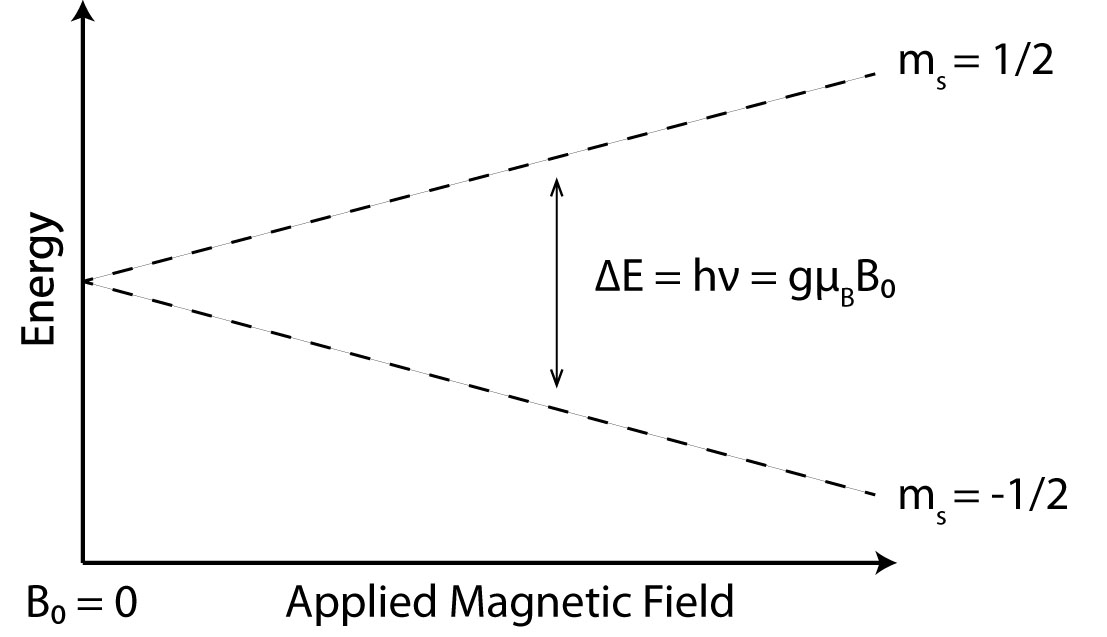
\includegraphics[scale=1]{Atom-ogMolekylefysik/billeder/Zeeman_Effect.jpg}
    \caption{opsplitningen af grundtilstandsenergien i hydrogenatomet, som konsekvens af Zeeman effekten}
    \label{fig:amo:vektor-projektion}
\end{figure}\\
Herfra kan man så inkludere kernens spin ved at gå over til at beskrive atomets totale angulære moment $F=J+I$, hvilket kan beskrives på samme måde som vi gjorde da vi udledte Zeeman opsplitningen for $J$ kvantetallene, dette er dog relativt simpelt, da man bare bruger samme metode som før og så ender med at få en $g_F$ faktor som på samme måde måde som $g_j$ faktoren vil indeholde en helvedes masse konstanter.


\end{document}